% =====================================================================
%  Capítulo 13. Valor en riesgo, déficit esperado y valores extremos
% =====================================================================
\part{Riesgo, valoración y temas avanzados}
\chapter[Valor en riesgo y valores extremos]{Valor en riesgo, déficit esperado y teoría de valores extremos}\label{cap:var_riesgo}

\section*{Objetivos de aprendizaje}
Al terminar este capítulo, el lector podrá:
\begin{enumerate}[label=\arabic*.,leftmargin=*]
  \item Definir el valor en riesgo (VaR) y el déficit esperado (ES), calcularlos con modelos normales, $t$ de
        Student, históricos y condicionales, y explicar por qué el VaR no es una medida coherente.
  \item Evaluar un modelo de VaR con las pruebas de Kupiec y Christoffersen y con el semáforo de Basilea.
  \item Modelar la cola de las pérdidas con la distribución de Pareto generalizada y derivar el VaR y el ES
        que implica.
  \item Calcular el riesgo a varios días y reconocer los límites de la regla de la raíz del tiempo.
\end{enumerate}

\section*{Motivación}
Un banco, un fondo de pensiones o una tesorería corporativa necesitan responder una pregunta concreta: ¿cuánto
podemos perder mañana en un mal día? El \emph{valor en riesgo}, popularizado por J.\,P.~Morgan en los noventa y
adoptado por el Comité de Basilea para fijar el capital de los bancos, responde con un cuantil de la distribución
de pérdidas. Pero un cuantil no dice nada sobre lo que ocurre más allá de él, y las crisis financieras ocurren
precisamente allí. Este capítulo reúne lo aprendido sobre colas gruesas (Capítulo~\ref{cap:hechos}) y volatilidad
condicional (Capítulos~\ref{cap:garch} y~\ref{cap:asimetria}) para medir, evaluar y modelar el riesgo extremo.

\paragraph{Datos del capítulo.} Rendimientos logarítmicos diarios del S\&P 500 (1999--2018) y del Brent
(1987--2026). Trabajamos con la pérdida $L_t=-r_t$, en porcentaje: una pérdida positiva es una caída del precio.

% ---------------------------------------------------------------------
\section{Valor en riesgo y déficit esperado}
% ---------------------------------------------------------------------

\begin{definicion}[VaR y ES]
Sea $L$ la pérdida de una posición en un horizonte dado y $p\in(0,1)$ un nivel de confianza (típicamente
$0{,}95$ o $0{,}99$). El \emph{valor en riesgo} es el cuantil $p$ de la pérdida,
\[
  \mathrm{VaR}_p=\inf\{\ell:\ \Pr(L\le\ell)\ge p\},
\]
y el \emph{déficit esperado} (\emph{expected shortfall}) es la pérdida media cuando se supera el VaR:
\[
  \mathrm{ES}_p=\E\bigl[L\mid L\ge\mathrm{VaR}_p\bigr]=\frac{1}{1-p}\int_p^1\mathrm{VaR}_u\,du .
\]
\end{definicion}

Un VaR al 99\,\% de 3\,\% a un día significa que, en promedio, uno de cada cien días la pérdida superará el 3\,\%. El
ES dice cuánto se pierde en promedio en esos días. Desde 2016, las reglas de Basilea para el riesgo de mercado
(\emph{Fundamental Review of the Trading Book}) usan el ES al 97,5\,\% en lugar del VaR al 99\,\%.

\begin{proposicion}[VaR y ES normales]\label{prop:esnormal}
Si $r\sim N(\mu,\sigma^2)$ y $L=-r$, con $z_p=\Phi^{-1}(p)$,
\[
  \mathrm{VaR}_p=-\mu+\sigma z_p,\qquad \mathrm{ES}_p=-\mu+\sigma\,\frac{\phi(z_p)}{1-p}.
\]
\end{proposicion}

\begin{proof}
La pérdida es $L=-\mu+\sigma Z$ con $Z\sim N(0,1)$, que es creciente en $Z$, así que su cuantil $p$ es
$-\mu+\sigma z_p$. Para el ES basta calcular $\E[Z\mid Z\ge z_p]$. Como $\phi'(z)=-z\phi(z)$:
\begin{align*}
  \E[Z\mid Z\ge z_p] &= \frac{1}{\Pr(Z\ge z_p)}\int_{z_p}^{\infty}z\,\phi(z)\,dz\\
                     &= \frac{1}{1-p}\Bigl[-\phi(z)\Bigr]_{z_p}^{\infty}\\
                     &= \frac{1}{1-p}\bigl(0+\phi(z_p)\bigr)\\
                     &= \frac{\phi(z_p)}{1-p}.
\end{align*}
Entonces $\mathrm{ES}_p=-\mu+\sigma\,\E[Z\mid Z\ge z_p]=-\mu+\sigma\phi(z_p)/(1-p)$.
\end{proof}

Con $p=0{,}99$, $z_p=2{,}3263$ y $\phi(z_p)/(1-p)=2{,}6652$: el ES normal es apenas un 15\,\% mayor que el VaR. Con
una $t$ de Student estandarizada de 4 grados de libertad, el VaR al 99\,\% es $2{,}65$ y el ES $3{,}69$, un 39\,\% mayor
(Figura~\ref{fig:vares}). Para la $t$ estandarizada, con $q=t_\nu^{-1}(p)$ y $c=\sqrt{(\nu-2)/\nu}$, un cálculo
similar da
\[
  \mathrm{VaR}_p=-\mu+\sigma\,c\,q,\qquad
  \mathrm{ES}_p=-\mu+\sigma\,c\,\frac{f_\nu(q)}{1-p}\cdot\frac{\nu+q^2}{\nu-1},
\]
donde $f_\nu$ es la densidad de la $t_\nu$.

\begin{figure}[ht]
\centering
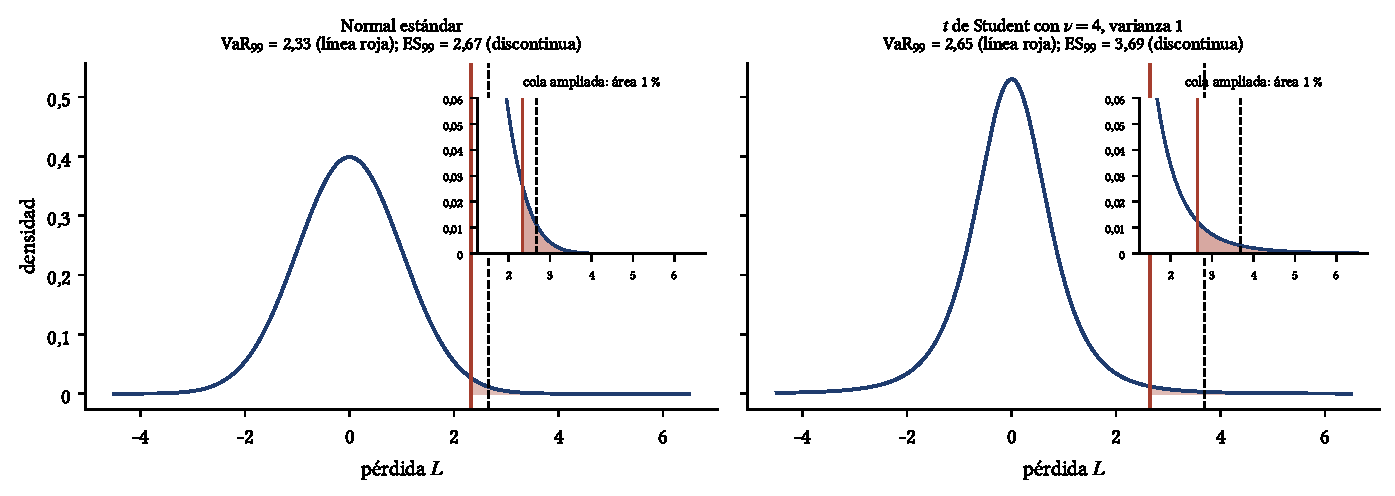
\includegraphics[width=\linewidth]{graficos/cap13_fig_var_es.pdf}
\caption{VaR y ES al 99\,\% para una pérdida normal estándar y para una $t$ de Student con varianza 1. El área
sombreada a la derecha del VaR es el 1\,\%; el ES es su centro de gravedad. Con colas gruesas el VaR sube poco, pero
el ES sube mucho.}
\label{fig:vares}
\end{figure}

\subsection{¿Es el VaR una buena medida de riesgo?}

Artzner, Delbaen, Eber y Heath (1999) propusieron cuatro propiedades que debería cumplir una medida de riesgo
\emph{coherente} $\rho$: monotonía, invarianza ante traslaciones, homogeneidad positiva y
\emph{subaditividad}, $\rho(L_1+L_2)\le\rho(L_1)+\rho(L_2)$, que formaliza que diversificar no aumenta el riesgo.
El ES es coherente; el VaR no siempre es subaditivo.

\begin{ejemplo}[El VaR castiga la diversificación]\label{ej:subaditivo}
Dos bonos independientes pagan 100 o, con probabilidad 4\,\%, nada. Para cada uno, la probabilidad de perder es
$0{,}04<0{,}05$, de modo que $\mathrm{VaR}_{0{,}95}=0$. Para la cartera con ambos,
\begin{align*}
  \Pr(\text{al menos un incumplimiento}) &= 1-0{,}96^2\\
                                         &= 0{,}0784>0{,}05,
\end{align*}
así que el VaR al 95\,\% de la cartera es una pérdida de 100, mayor que $0+0$. Según el VaR, diversificar
\emph{aumentó} el riesgo, porque el VaR ignora el tamaño de las pérdidas más allá del cuantil.
\end{ejemplo}

\subsection{Métodos de estimación}

\begin{itemize}[leftmargin=*]
  \item \textbf{Paramétrico incondicional}: se supone una distribución (normal, $t$) con parámetros constantes.
  \item \textbf{Simulación histórica (HS)}: el VaR es el cuantil empírico de las últimas $n$ pérdidas (por ejemplo,
        $n=500$); el ES, el promedio de las que lo superan. No supone una distribución, pero reacciona tarde a los
        cambios de volatilidad y no puede ir más allá de lo observado.
  \item \textbf{Paramétrico condicional}: $\mathrm{VaR}_{t}=-\mu_t+\sigma_t q_p$, con $\sigma_t$ de un EWMA o un
        GARCH estimado con datos hasta $t-1$.
  \item \textbf{Simulación histórica filtrada (FHS)}: se remuestrean los residuos estandarizados de un GARCH y se
        reescalan con la volatilidad actual (Barone-Adesi y Giannopoulos, 2001). Combina la dinámica del GARCH
        con la forma empírica de las colas.
\end{itemize}

% ---------------------------------------------------------------------
\section{Pruebas retrospectivas}
% ---------------------------------------------------------------------

Sea $I_t=\mathbf 1(L_t>\mathrm{VaR}_t)$ el indicador de una \emph{excepción}. Si el modelo es correcto, los $I_t$
son i.i.d.\ Bernoulli con probabilidad $1-p$ (Christoffersen, 1998): la tasa de excepciones debe ser la correcta
(\emph{cobertura incondicional}) y las excepciones no deben agruparse (\emph{independencia}).

\begin{proposicion}[Prueba de Kupiec]\label{prop:kupiec}
Con $n$ días y $k$ excepciones, sea $q=1-p$ y $\hat\pi=k/n$. El estadístico de razón de verosimilitudes de
$H_0:\Pr(I_t=1)=q$ es
\[
  LR_{uc}=-2\Bigl[(n-k)\ln(1-q)+k\ln q-(n-k)\ln(1-\hat\pi)-k\ln\hat\pi\Bigr]\ \xrightarrow{d}\ \chi^2_1 .
\]
\end{proposicion}

\begin{proof}
Bajo independencia, la verosimilitud de la secuencia de excepciones con probabilidad $\pi$ es
\begin{align*}
  \mathcal L(\pi) &= \prod_{t=1}^{n}\pi^{I_t}(1-\pi)^{1-I_t}\\
                  &= \pi^{k}(1-\pi)^{n-k}.
\end{align*}
Su logaritmo, $\ell(\pi)=k\ln\pi+(n-k)\ln(1-\pi)$, se maximiza en
\begin{align*}
  \ell'(\pi) &= \frac{k}{\pi}-\frac{n-k}{1-\pi}=0,\\
  k(1-\pi)   &= (n-k)\pi,\\
  \hat\pi    &= \frac kn .
\end{align*}
La razón de verosimilitudes es $-2[\ell(q)-\ell(\hat\pi)]$, que es la fórmula del enunciado, con una restricción.
\end{proof}

La prueba de \emph{independencia} de Christoffersen (1998) modela $I_t$ como una cadena de Markov con
probabilidades $\pi_{01}=\Pr(I_t=1\mid I_{t-1}=0)$ y $\pi_{11}=\Pr(I_t=1\mid I_{t-1}=1)$, estimadas con los conteos
de transiciones $n_{ij}$, y contrasta $\pi_{01}=\pi_{11}$:
\[
  LR_{ind}=-2\Bigl[\ell(\hat\pi_1)-\ell(\hat\pi_{01},\hat\pi_{11})\Bigr]\xrightarrow{d}\chi^2_1,
\]
donde $\ell(\hat\pi_1)=(n_{00}+n_{10})\ln(1-\hat\pi_1)+(n_{01}+n_{11})\ln\hat\pi_1$ y
$\ell(\hat\pi_{01},\hat\pi_{11})=n_{00}\ln(1-\hat\pi_{01})+n_{01}\ln\hat\pi_{01}+n_{10}\ln(1-\hat\pi_{11})+n_{11}\ln\hat\pi_{11}$.
La prueba de \emph{cobertura condicional} suma ambas: $LR_{cc}=LR_{uc}+LR_{ind}\sim\chi^2_2$.

\paragraph{El semáforo de Basilea.} Los supervisores bancarios cuentan las excepciones del VaR al 99\,\% en los últimos
250 días. Con 0 a 4 el modelo está en zona \emph{verde}; con 5 a 9, en zona \emph{amarilla}, y el multiplicador del
capital sube de 3 a entre 3,40 y 3,85; con 10 o más, en zona \emph{roja}, y el multiplicador es 4. Las fronteras
salen de la distribución binomial: si el modelo es correcto, $\Pr(X\le4)=0{,}8922$ y $\Pr(X\le9)=0{,}9997$ con
$X\sim\mathrm{Bin}(250;\ 0{,}01)$.

% ---------------------------------------------------------------------
\section{Teoría de valores extremos}
% ---------------------------------------------------------------------

Para el VaR al 99,9\,\% de una cartera, o para una pérdida que ocurre una vez cada diez años, los datos históricos
son escasos y la normal subestima el riesgo. La teoría de valores extremos ofrece un modelo para la cola que no
depende de la distribución completa.

\begin{definicion}[Distribución de Pareto generalizada]
La GPD con parámetro de forma $\xi$ y escala $\beta>0$ tiene función de distribución
\[
  G_{\xi,\beta}(y)=\begin{cases}
     1-\bigl(1+\xi y/\beta\bigr)^{-1/\xi}, & \xi\ne0,\\[2pt]
     1-e^{-y/\beta}, & \xi=0,
  \end{cases}
\]
para $y\ge0$ (y $y\le-\beta/\xi$ si $\xi<0$).
\end{definicion}

El \emph{teorema de Pickands-Balkema-de Haan} dice que, para una clase muy amplia de distribuciones, los excesos
$Y=L-u$ sobre un umbral $u$ alto, condicionados a $L>u$, se distribuyen aproximadamente como una GPD. El índice de
cola $\xi$ determina el tipo: $\xi>0$ para colas gruesas de tipo Pareto (como la $t$, con $\xi=1/\nu$), $\xi=0$ para
colas exponenciales (como la normal) y $\xi<0$ para distribuciones acotadas. La Figura~\ref{fig:gpd} muestra que las
tres formas se distinguen en la cola: en escala logarítmica, la exponencial es una recta, la de $\xi>0$ cae más
despacio y la de $\xi<0$ llega a un máximo finito.

\begin{proposicion}[VaR y ES con la cola GPD]\label{prop:gpdvar}
Sea $u$ un umbral, $n$ el número de observaciones y $N_u$ el de pérdidas mayores que $u$. Si los excesos siguen
una GPD con $0<\xi<1$, para $p>1-N_u/n$:
\begin{align*}
  \mathrm{VaR}_p &= u+\frac{\beta}{\xi}\Bigl[\Bigl(\frac{n}{N_u}(1-p)\Bigr)^{-\xi}-1\Bigr],\\
  \mathrm{ES}_p  &= \frac{\mathrm{VaR}_p}{1-\xi}+\frac{\beta-\xi u}{1-\xi}.
\end{align*}
\end{proposicion}

\begin{proof}
Para $x>u$, la probabilidad de la cola se descompone como
\begin{align*}
  \Pr(L>x) &= \Pr(L>u)\,\Pr(L>x\mid L>u)\\
           &\approx \frac{N_u}{n}\Bigl(1+\xi\,\frac{x-u}{\beta}\Bigr)^{-1/\xi}.
\end{align*}
El VaR resuelve $\Pr(L>x)=1-p$:
\begin{align*}
  \Bigl(1+\xi\,\frac{x-u}{\beta}\Bigr)^{-1/\xi} &= \frac{n}{N_u}(1-p),\\
  1+\xi\,\frac{x-u}{\beta} &= \Bigl(\frac{n}{N_u}(1-p)\Bigr)^{-\xi},\\
  x &= u+\frac\beta\xi\Bigl[\Bigl(\frac{n}{N_u}(1-p)\Bigr)^{-\xi}-1\Bigr].
\end{align*}
Para el ES usamos la \emph{media de los excesos} de la GPD, que es lineal en el umbral: si los excesos sobre $u$ son
GPD$(\xi,\beta)$, los excesos sobre $v>u$ son GPD$(\xi,\beta+\xi(v-u))$, y la media de una GPD es escala$/(1-\xi)$. Así
\begin{align*}
  e(v)=\E[L-v\mid L>v] &= \frac{\beta+\xi(v-u)}{1-\xi}.
\end{align*}
Con $v=\mathrm{VaR}_p$:
\begin{align*}
  \mathrm{ES}_p &= \mathrm{VaR}_p+e(\mathrm{VaR}_p)\\
                &= \mathrm{VaR}_p+\frac{\beta+\xi\,\mathrm{VaR}_p-\xi u}{1-\xi}\\
                &= \frac{(1-\xi)\mathrm{VaR}_p+\xi\,\mathrm{VaR}_p}{1-\xi}+\frac{\beta-\xi u}{1-\xi}\\
                &= \frac{\mathrm{VaR}_p}{1-\xi}+\frac{\beta-\xi u}{1-\xi}. && \qedhere
\end{align*}
\end{proof}

La linealidad de $e(v)$ da una herramienta gráfica para elegir el umbral: el gráfico de la media empírica de los
excesos debe ser aproximadamente una recta con pendiente $\xi/(1-\xi)$ por encima de un buen umbral (Figura~\ref{fig:gpd},
derecha). Elegir $u$ implica un equilibrio: un umbral bajo da muchos excesos pero quizá no GPD (sesgo); uno alto,
pocos excesos (varianza). En la práctica se usa un cuantil entre el 90 y el 97,5\,\% y se verifica la estabilidad
de $\hat\xi$. Los parámetros se estiman por máxima verosimilitud con la log-verosimilitud
\[
  \ell(\xi,\beta)=-N_u\ln\beta-\Bigl(1+\frac1\xi\Bigr)\sum_{i=1}^{N_u}\ln\Bigl(1+\frac{\xi y_i}{\beta}\Bigr).
\]

\begin{figure}[ht]
\centering
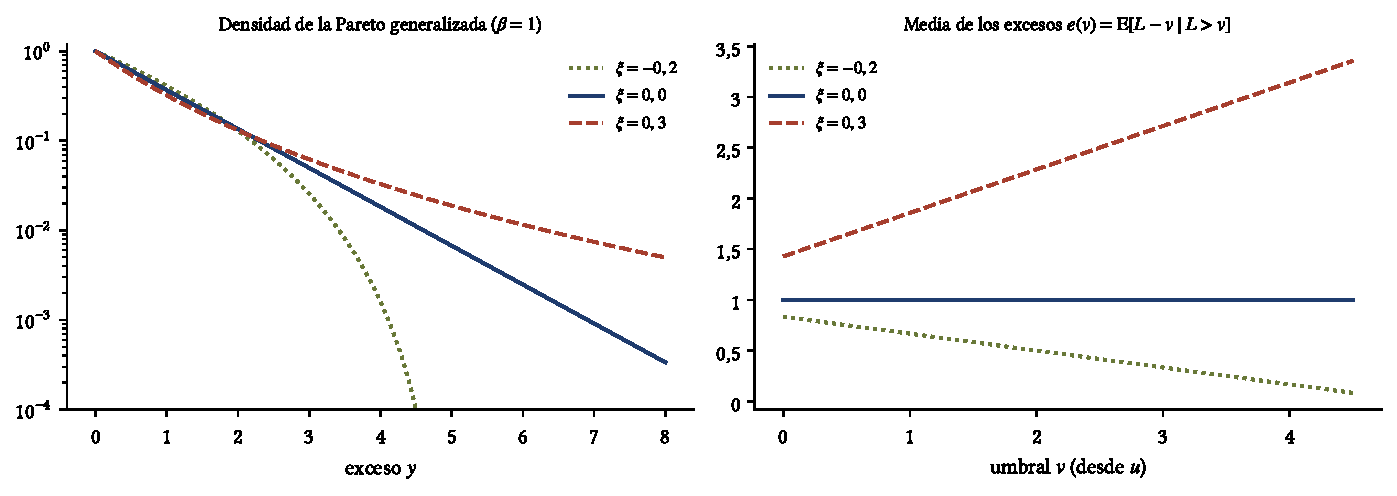
\includegraphics[width=\linewidth]{graficos/cap13_fig_gpd.pdf}
\caption{Izquierda: densidad de la GPD con $\beta=1$ en escala logarítmica. Derecha: su función de media de los
excesos, creciente si $\xi>0$, constante si $\xi=0$ y decreciente si $\xi<0$.}
\label{fig:gpd}
\end{figure}

% ---------------------------------------------------------------------
\section{Riesgo a varios días}
% ---------------------------------------------------------------------

La regulación pide a veces el VaR a 10 días. La \emph{regla de la raíz del tiempo},
$\mathrm{VaR}^{(10)}=\sqrt{10}\,\mathrm{VaR}^{(1)}$, supone que los rendimientos son i.i.d.\ normales con media
cero. Falla por tres razones: la volatilidad revierte a su media (Proposición~\ref{prop:garchpron}), así que la regla
sobreestima el riesgo cuando la volatilidad está alta y lo subestima cuando está baja; la suma de rendimientos con
colas gruesas tiene colas menos gruesas que cada sumando, así que multiplicar el cuantil de un día por $\sqrt{10}$
exagera la cola; y la retroalimentación del GARCH (un día malo eleva la volatilidad de los siguientes) engorda la
cola de las pérdidas acumuladas. La simulación histórica filtrada captura los tres efectos.

% ---------------------------------------------------------------------
\section{Ejercicios resueltos}
% ---------------------------------------------------------------------

\begin{ejresuelto}{VaR y ES incondicionales}\label{ej:varincond}
\enunciado Calcule el VaR y el ES a un día al 95 y al 99\,\% para el S\&P 500 y el Brent con la normal, la $t$ de Student
(con $\nu$ elegido para reproducir la curtosis muestral) y la simulación histórica, y la frecuencia con que cada VaR
fue superado en la muestra.

\solucion
\paso{Paso 1. La $t$ por momentos.} Como la curtosis de la $t_\nu$ es $\kappa=3+6/(\nu-4)$, despejando
\begin{align*}
  \nu &= 4+\frac{6}{\kappa-3}.
\end{align*}
Para el S\&P 500, $\kappa=11{,}17$ y $\nu=4+6/8{,}17=4{,}734$; para el Brent, $\kappa=55{,}97$ y $\nu=4{,}113$.

\paso{Paso 2. VaR normal del S\&P 500 al 99\,\%.} Con $\hat\mu=0{,}0142$ y $\hat\sigma=1{,}2038$:
\begin{align*}
  \mathrm{VaR}_{0{,}99} &= -0{,}0142+1{,}2038\times2{,}3263=2{,}786,\\
  \mathrm{ES}_{0{,}99}  &= -0{,}0142+1{,}2038\times2{,}6652=3{,}194 .
\end{align*}

\paso{Paso 3. Comparación.}
\begin{center}\small
\begin{tabular}{@{}llrrrrrr@{}}
\toprule
 & & \multicolumn{3}{c}{S\&P 500} & \multicolumn{3}{c}{Brent} \\
\cmidrule(lr){3-5}\cmidrule(lr){6-8}
Nivel & Modelo & VaR & ES & Frec. & VaR & ES & Frec. \\
\midrule
95\,\% & normal    & 1,966 & 2,469 & 4,63\,\% & 4,429 & 5,559 & 3,26\,\% \\
       & $t$       & 1,852 & 2,690 & 5,21\,\% & 4,080 & 6,099 & 4,19\,\% \\
       & histórico & 1,882 & 2,910 & 5,01\,\% & 3,799 & 6,133 & 5,00\,\% \\
99\,\% & normal    & 2,786 & 3,194 & 1,83\,\% & 6,271 & 7,188 & 1,32\,\% \\
       & $t$       & 3,138 & 4,203 & 1,27\,\% & 7,134 & 9,873 & 0,99\,\% \\
       & histórico & 3,362 & 4,814 & 1,01\,\% & 7,120 & 11,289 & 1,01\,\% \\
\bottomrule
\end{tabular}
\end{center}
Al 95\,\% los tres modelos se parecen y la normal incluso \emph{sobreestima} el VaR (la cola empieza a engordar más
lejos). Al 99\,\% la normal subestima: su VaR del S\&P 500 se supera el 1,83\,\% de los días, casi el doble de lo
previsto, y su ES es un tercio menor que el histórico. La Figura~\ref{fig:colas} muestra por qué: en escala
logarítmica, la cola normal se hunde mientras la empírica sigue casi recta.

\codigoweb{cap13_ej01}
\salidaR{cap13_ej01_R.txt}
\lectura{cap13_ej01}

\RvsPy El cuantil empírico usa interpolación lineal en ambos lenguajes: \texttt{quantile(..., type = 7)} en R y el
método por omisión de \texttt{np.quantile}. Con otros métodos el VaR histórico cambia en la tercera cifra. En R, los
nombres de lista con tilde (\texttt{"histórico"}) deben ir entre comillas.

\begin{figure}[ht]
\centering
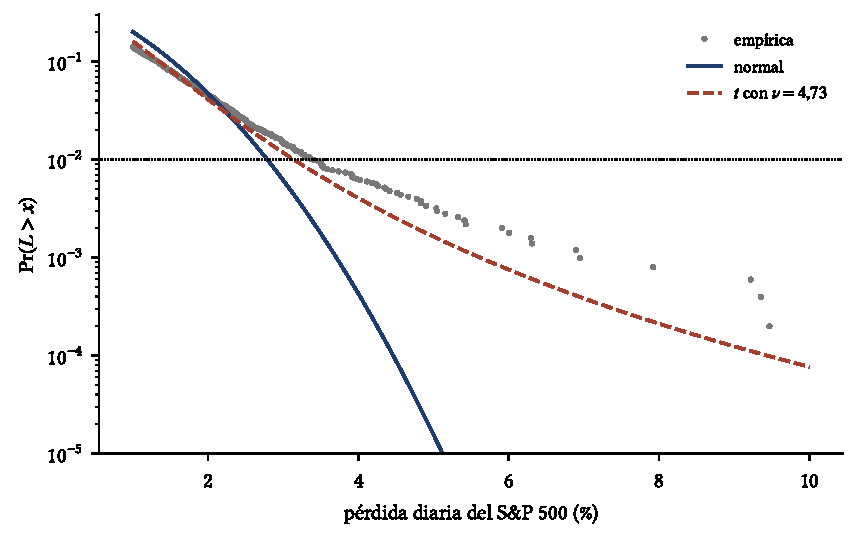
\includegraphics[width=0.7\linewidth]{graficos/cap13_ej01_colas.pdf}
\caption{Probabilidad de que la pérdida diaria del S\&P 500 supere $x$: empírica, normal y $t$ de Student. La línea
horizontal marca el 1\,\%.}
\label{fig:colas}
\end{figure}

\begin{conclusion}
La normal es aceptable al 95\,\%, pero subestima el riesgo al 99\,\% y, sobre todo, el déficit esperado. Para el Brent,
cuya cola es mucho más gruesa, el ES histórico al 99\,\% es un 57\,\% mayor que el normal.
\end{conclusion}
\end{ejresuelto}

\begin{ejresuelto}{Prueba retrospectiva del VaR del S\&P 500}\label{ej:backtest}
\enunciado Calcule cada día de 2001 a 2018 el VaR al 99\,\% a un día del S\&P 500 con: (i) simulación histórica con 500
días; (ii) EWMA normal ($\lambda=0{,}94$, media cero); (iii) GARCH(1,1)-$t$ reestimado cada enero con todos los datos
anteriores. Aplique las pruebas de Kupiec, Christoffersen y de cobertura condicional.

\solucion
\paso{Paso 1. Resultados.} En 4\,527 días se esperan $45{,}3$ excepciones:
\begin{center}\small
\begin{tabular}{@{}lrrrrrr@{}}
\toprule
Modelo & VaR medio & Excepciones & Tasa & $LR_{uc}$ & $LR_{ind}$ & $LR_{cc}$ \\
\midrule
HS-500      & 3,016 & 73 & 1,61\,\% & 14,47 & 10,71 & 25,18 \\
EWMA normal & 2,375 & 96 & 2,12\,\% & 43,44 & 3,25 & 46,69 \\
GARCH-$t$   & 2,585 & 65 & 1,44\,\% & 7,65 & 3,01 & 10,66 \\
\bottomrule
\end{tabular}
\end{center}

\paso{Paso 2. Kupiec para el GARCH-$t$.} Con $\hat\pi=65/4\,527=0{,}01436$:
\begin{align*}
  \ell(0{,}01) &= 4\,462\ln0{,}99+65\ln0{,}01=-344{,}18,\\
  \ell(\hat\pi) &= 4\,462\ln0{,}98564+65\ln0{,}01436=-340{,}35,\\
  LR_{uc} &= -2\,(-344{,}18+340{,}35)=7{,}65,
\end{align*}
con valor $p$ de $0{,}006$: se rechaza la cobertura correcta, aunque el GARCH-$t$ es el mejor de los tres.

\paso{Paso 3. Interpretación.} Los tres modelos tienen más excepciones de las debidas. La EWMA normal es la peor en
cobertura (96): la normal subestima la cola. La simulación histórica tiene el VaR medio más alto, pero aun así
falla 73 veces porque sus excepciones se concentran: 21 en 2008 (de 253 días), cuando la ventana de 500 días todavía
reflejaba la calma de 2006--2007 (Figura~\ref{fig:backtest}). Por eso es la única que rechaza la independencia
($LR_{ind}=10{,}71$, $p=0{,}001$). Los modelos condicionales reaccionan en días: en 2008 la EWMA tuvo 9 excepciones y
el GARCH-$t$, 7.

\codigoweb{cap13_ej02}
\salidaR{cap13_ej02_R.txt}
\lectura{cap13_ej02}

\RvsPy El GARCH-$t$ se reestima 18 veces con la función \texttt{garch\_fit} del Capítulo~\ref{cap:garch}; con los
parámetros de cada año, la recursión corre sobre toda la serie y se toman las varianzas de ese año, que solo
dependen de datos anteriores. Las excepciones coinciden una a una entre R y Python. Las series de VaR se guardan en
un CSV para el ejercicio siguiente; en R hay que pasar \texttt{check.names = FALSE} a \texttt{data.frame} para que
nombres como \texttt{HS-500} no se conviertan en \texttt{HS.500}.

\begin{figure}[ht]
\centering
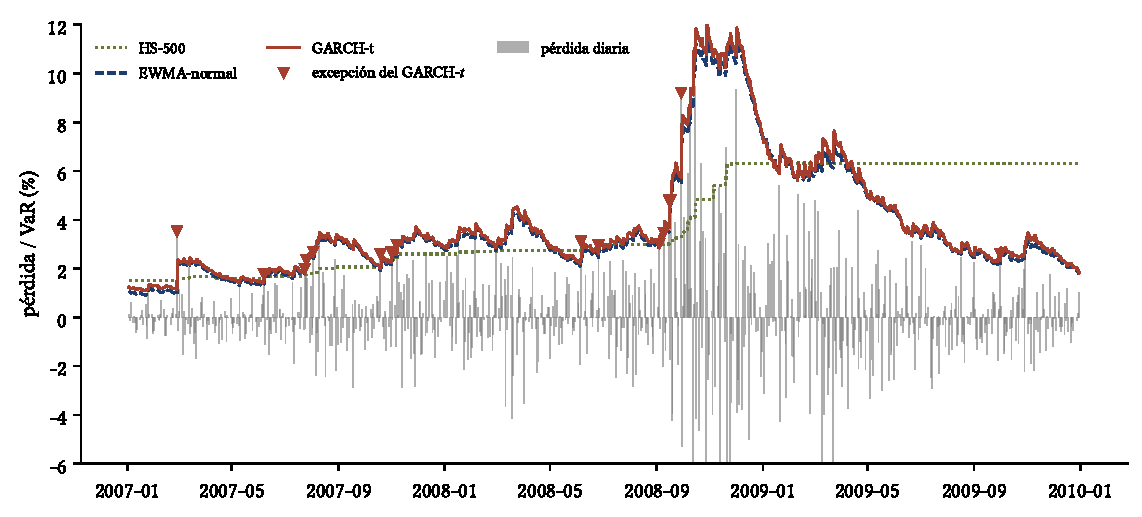
\includegraphics[width=0.92\linewidth]{graficos/cap13_ej02_backtest.pdf}
\caption{Pérdidas diarias del S\&P 500 y VaR al 99\,\% de los tres modelos en 2007--2009. La simulación histórica
(punteada) tarda meses en reaccionar a la crisis; los triángulos son las excepciones del GARCH-$t$.}
\label{fig:backtest}
\end{figure}

\begin{conclusion}
Los modelos condicionales siguen a la volatilidad, y el de colas $t$ es el que más se acerca a la cobertura correcta.
La simulación histórica falla en el peor momento: cuando empieza una crisis.
\end{conclusion}
\end{ejresuelto}

\begin{ejresuelto}{El semáforo de Basilea}\label{ej:semaforo}
\enunciado Con los VaR del Ejercicio~\ref{ej:backtest}, cuente las excepciones de cada año calendario y asigne la zona
del semáforo de Basilea.

\solucion
\paso{Paso 1. Conteos.}
\begin{center}\small
\begin{tabular}{@{}lrrr|lrrr@{}}
\toprule
Año & HS & EWMA & GARCH-$t$ & Año & HS & EWMA & GARCH-$t$ \\
\midrule
2001 & 4 & 4 & 2 & 2010 & 0 & 9 & 6 \\
2002 & 5 & 2 & 2 & 2011 & 5 & 6 & 6 \\
2003 & 1 & 1 & 0 & 2012 & 0 & 5 & 4 \\
2004 & 0 & 3 & 0 & 2013 & 0 & 5 & 3 \\
2005 & 2 & 3 & 0 & 2014 & 2 & 10 & 6 \\
2006 & 4 & 5 & 3 & 2015 & 6 & 6 & 4 \\
2007 & 11 & 12 & 8 & 2016 & 3 & 2 & 2 \\
2008 & 21 & 9 & 7 & 2017 & 0 & 4 & 3 \\
2009 & 0 & 2 & 1 & 2018 & 9 & 8 & 8 \\
\bottomrule
\end{tabular}
\end{center}

\paso{Paso 2. Zonas.} La simulación histórica pasa 12 años en verde, 4 en amarillo y 2 en rojo (2007 y 2008); la EWMA,
8, 8 y 2 (2007 y 2014); el GARCH-$t$, 12, 6 y ninguno en rojo. Con los recargos de Basilea, el multiplicador medio del
capital sería 3,231 para la simulación histórica, 3,369 para la EWMA y 3,203 para el GARCH-$t$.

\paso{Paso 3. Paradoja de la simulación histórica.} Fuera de las crisis, la simulación histórica casi nunca falla
(siete años con 0 o 1 excepción): su VaR es demasiado \emph{conservador} en la calma y demasiado \emph{laxo} al
inicio de una crisis. Un banco que la usara inmovilizaría capital de más casi siempre y caería en la zona roja cuando
más duele (Figura~\ref{fig:semaforo}).

\codigoweb{cap13_ej03}
\salidaR{cap13_ej03_R.txt}
\lectura{cap13_ej03}

\RvsPy Cada lenguaje lee el CSV que generó en el ejercicio anterior. Los recargos (0,40; 0,50; 0,65; 0,75 y 0,85 para 5 a 9
excepciones) se guardan en un vector indexado por el número de excepciones; en R los índices empiezan en 1, por eso
se usa \texttt{extra[k + 1]}.

\begin{figure}[ht]
\centering
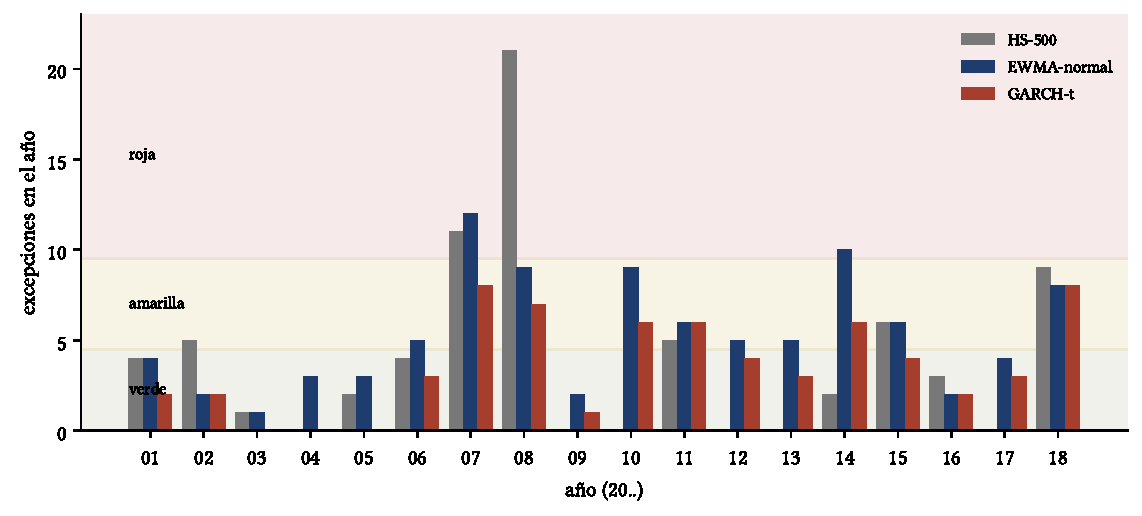
\includegraphics[width=0.92\linewidth]{graficos/cap13_ej03_semaforo.pdf}
\caption{Excepciones anuales del VaR al 99\,\% del S\&P 500 y zonas del semáforo de Basilea.}
\label{fig:semaforo}
\end{figure}

\begin{conclusion}
El GARCH-$t$ nunca habría llevado al banco a la zona roja en 18 años; la simulación histórica y la EWMA, dos veces
cada una. La prueba de Basilea es exigente con los modelos que no reaccionan a la volatilidad.
\end{conclusion}
\end{ejresuelto}

\begin{ejresuelto}{Valores extremos del Brent y del S\&P 500}\label{ej:evt}
\enunciado Estime una GPD para los excesos de las pérdidas diarias sobre los cuantiles 90, 95 y 97,5\,\%. Con el umbral del
95\,\%, calcule el VaR y el ES al 99; 99,5 y 99,9\,\% y compárelos con la normal, la $t$ y la simulación histórica.

\solucion
\paso{Paso 1. Estabilidad de $\hat\xi$.}
\begin{center}\small
\begin{tabular}{@{}lrrrr@{}}
\toprule
 & \multicolumn{2}{c}{Brent} & \multicolumn{2}{c}{S\&P 500} \\
\cmidrule(lr){2-3}\cmidrule(lr){4-5}
Umbral & $\hat\xi$ (ee) & $N_u$ & $\hat\xi$ (ee) & $N_u$ \\
\midrule
90\,\%   & 0,270 (0,039) & 912 & 0,155 (0,050) & 503 \\
95\,\%   & 0,371 (0,063) & 456 & 0,168 (0,072) & 252 \\
97,5\,\% & 0,445 (0,101) & 228 & 0,236 (0,121) & 126 \\
\bottomrule
\end{tabular}
\end{center}
La cola del Brent es mucho más gruesa ($\hat\xi\approx0{,}37$, equivalente a una $t$ con menos de 3 grados de
libertad) que la del S\&P 500 ($\hat\xi\approx0{,}17$). En el Brent $\hat\xi$ crece con el umbral: la cola extrema
está dominada por unos pocos días (abril de 2020, 1991, 2026).

\paso{Paso 2. VaR con la GPD.} Para el Brent, $u=3{,}799$, $N_u=456$, $n=9\,121$, $\hat\xi=0{,}3706$ y
$\hat\beta=1{,}4650$. Al 99\,\%:
\begin{align*}
  \frac{n}{N_u}(1-p) &= 20{,}002\times0{,}01=0{,}20002,\\
  0{,}20002^{-0{,}3706} &= 1{,}8156,\\
  \mathrm{VaR}_{0{,}99} &= 3{,}799+\frac{1{,}4650}{0{,}3706}\,(1{,}8156-1)=7{,}023,\\
  \mathrm{ES}_{0{,}99} &= \frac{7{,}023}{0{,}6294}+\frac{1{,}4650-0{,}3706\times3{,}799}{0{,}6294}=11{,}16+0{,}09=11{,}25 .
\end{align*}

\paso{Paso 3. Comparación (Brent).}
\begin{center}\small
\begin{tabular}{@{}lrrrrrrrr@{}}
\toprule
 & \multicolumn{2}{c}{GPD} & \multicolumn{2}{c}{Normal} & \multicolumn{2}{c}{$t$} & \multicolumn{2}{c}{Histórico} \\
\cmidrule(lr){2-3}\cmidrule(lr){4-5}\cmidrule(lr){6-7}\cmidrule(lr){8-9}
Nivel & VaR & ES & VaR & ES & VaR & ES & VaR & ES \\
\midrule
99\,\%   & 7,02 & 11,25 & 6,27 & 7,19 & 7,13 & 9,87 & 7,12 & 11,29 \\
99,5\,\% & 9,13 & 14,59 & 6,95 & 7,80 & 8,74 & 11,92 & 9,02 & 14,73 \\
99,9\,\% & 16,69 & 26,61 & 8,34 & 9,09 & 13,50 & 18,09 & 16,82 & 26,70 \\
\bottomrule
\end{tabular}
\end{center}
La GPD reproduce casi exactamente los cuantiles y ES empíricos incluso al 99,9\,\%, donde hay solo 9 observaciones. La
normal da un VaR al 99,9\,\% de la mitad del real, y un ES de un tercio. La $t$ por momentos mejora, pero se queda corta
porque su $\nu$ se calibró con la curtosis, que mide toda la distribución y no solo la cola (Figura~\ref{fig:evt}).

\codigoweb{cap13_ej04}
\salidaR{cap13_ej04_R.txt}
\lectura{cap13_ej04}

\RvsPy La verosimilitud de la GPD se maximiza con Nelder-Mead en ambos lenguajes; R y Python coinciden hasta la
sexta decimal, y \texttt{genpareto.fit(y, floc=0)} de \texttt{scipy} da el mismo $\hat\xi=0{,}3705$. Ojo con la
parametrización: en \texttt{scipy} el parámetro de forma se llama \texttt{c} y coincide con $\xi$.

\begin{figure}[ht]
\centering
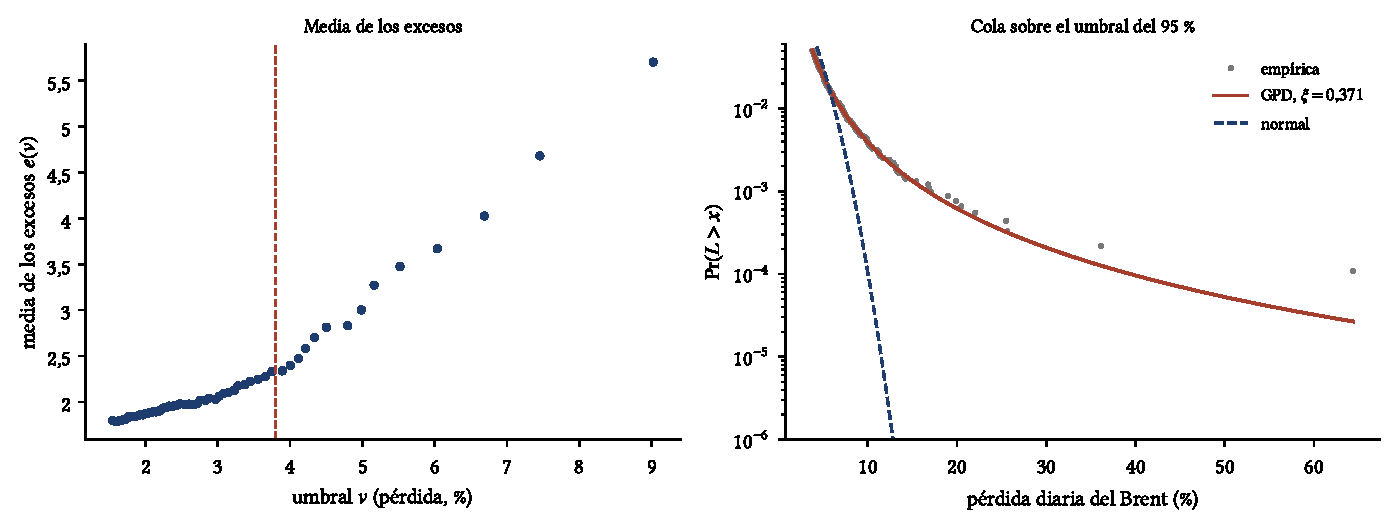
\includegraphics[width=\linewidth]{graficos/cap13_ej04_evt.pdf}
\caption{Brent. Izquierda: media empírica de los excesos; por encima del umbral del 95\,\% (línea discontinua) crece
aproximadamente en línea recta. Derecha: probabilidad empírica de la cola frente a la GPD ajustada y a la normal.}
\label{fig:evt}
\end{figure}

\begin{conclusion}
La teoría de valores extremos permite estimar cuantiles muy altos con un modelo apoyado en la teoría, y no solo en
unos pocos datos. Para el petróleo, la diferencia entre la normal y la GPD al 99,9\,\% es de más de 8 puntos
porcentuales de pérdida diaria.
\end{conclusion}
\end{ejresuelto}

\begin{ejresuelto}{VaR a 10 días del Brent}\label{ej:var10}
\enunciado Con un GARCH(1,1)-$t$ estimado para el Brent, calcule el VaR al 99\,\% a 10 días el 31 de diciembre de 2019 (calma)
y el 3 de noviembre de 2026 (alta volatilidad) con: (i) la regla de la raíz aplicada al VaR $t$ a un día; (ii) la
varianza acumulada del GARCH con un cuantil normal; (iii) simulación histórica filtrada con 100\,000 trayectorias.

\solucion
\paso{Paso 1. Varianza acumulada.} Por el Corolario~\ref{cor:varH}, con $\hat\phi=0{,}9955$ y la varianza de largo
plazo de $13{,}29$: el 31 de diciembre de 2019 la varianza de mañana era $1{,}519^2=2{,}31$, muy por debajo, y la
desviación estándar acumulada a 10 días es $5{,}03$\,\%, algo más que $\sqrt{10}\times1{,}519=4{,}80$\,\%. El 3 de noviembre
de 2026 era $4{,}762^2=22{,}68$, por encima, y la acumulada es $15{,}00$\,\%, algo menos que $\sqrt{10}\times4{,}762=15{,}06$\,\%.

\paso{Paso 2. Resultados.}
\begin{center}\small
\begin{tabular}{@{}lrr@{}}
\toprule
VaR al 99\,\% a 10 días & 2019-12-31 & 2026-11-03 \\
\midrule
VaR $t$ a 1 día & 3,89 & 12,31 \\
Raíz del tiempo: $\sqrt{10}\times$VaR & 12,31 & 38,94 \\
Varianza GARCH acumulada, cuantil normal & 11,17 & 34,37 \\
Simulación filtrada (R) & 12,64 & 39,58 \\
Simulación filtrada (Python) & 12,97 & 39,07 \\
\bottomrule
\end{tabular}
\end{center}
El enfoque de la varianza acumulada con un cuantil normal es el más bajo: corrige la reversión a la media pero ignora
que la pérdida a 10 días sigue teniendo colas gruesas. La simulación filtrada da cifras parecidas a la regla de la raíz,
pero por razones distintas: la regla exagera la cola (multiplica un cuantil $t$ de un día) y la simulación la
reconstruye con la retroalimentación del GARCH, en la que un día malo eleva la volatilidad de los siguientes. El ES
simulado es de alrededor de 16\,\% en 2019 y de 49 a 50\,\% en 2026 (Figura~\ref{fig:var10}).

\codigoweb{cap13_ej05}
\salidaR{cap13_ej05_R.txt}
\lectura{cap13_ej05}

\RvsPy Los métodos analíticos coinciden en todas las cifras. La simulación difiere entre R y Python en torno al 2--3\,\%
porque cada lenguaje usa su propio generador de números aleatorios; la diferencia es grande para 100\,000
trayectorias porque la cola de la pérdida acumulada la dominan unos pocos residuos estandarizados extremos (como el
de abril de 2020), que se sortean con probabilidad $1/9\,121$ en cada día. Python vectoriza las trayectorias y R
recorre un bucle; con 100\,000 trayectorias, R tarda unos 15 segundos.

\begin{figure}[ht]
\centering
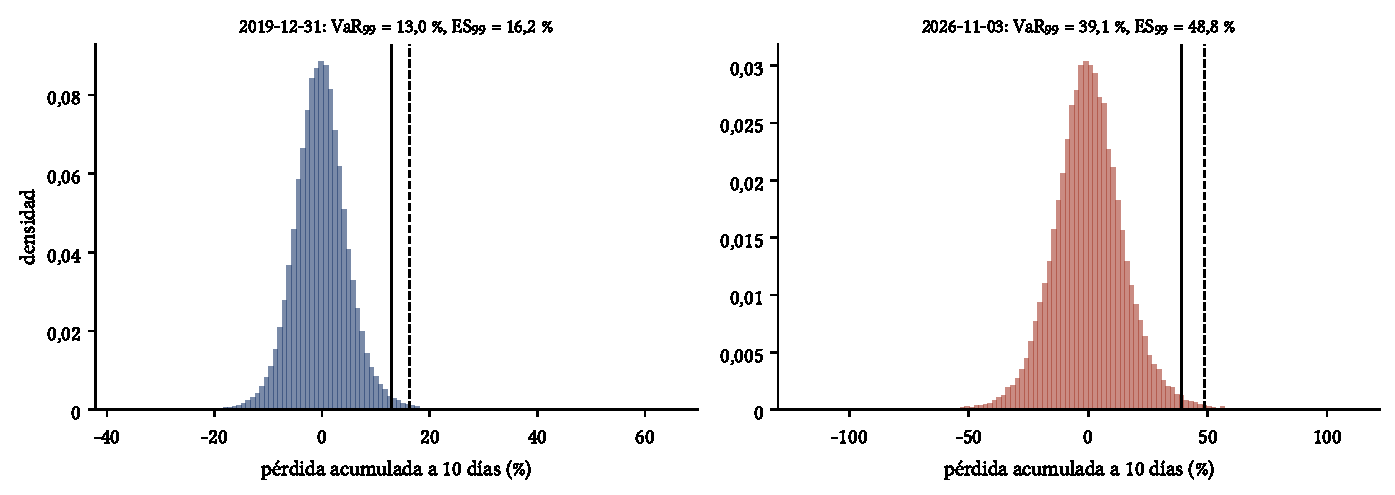
\includegraphics[width=\linewidth]{graficos/cap13_ej05_10dias.pdf}
\caption{Distribución simulada de la pérdida acumulada a 10 días del Brent, en calma y en alta volatilidad, con el VaR
(línea continua) y el ES (discontinua) al 99\,\%.}
\label{fig:var10}
\end{figure}

\begin{conclusion}
El riesgo a varios días depende del nivel de volatilidad de partida y de la forma de la cola, y la regla de la raíz
acierta en este caso por casualidad, al compensarse dos errores. La simulación filtrada es el método más completo,
pero su precisión en la cola extrema requiere muchas trayectorias.
\end{conclusion}
\end{ejresuelto}

% ---------------------------------------------------------------------
\section{Ejercicios propuestos}
% ---------------------------------------------------------------------

\begin{enumerate}[label=\textbf{\thechapter.\arabic*},leftmargin=*,itemsep=6pt]
  \item Un portafolio de 10 millones de soles tiene rendimiento diario normal con media 0 y desviación 1,5\,\%. Calcule el VaR
  y el ES al 99\,\% a un día y a 10 días (regla de la raíz). \textit{Respuesta: 349\,000 y 400\,000 soles; 1\,103\,000 y 1\,264\,000.}

  \item Demuestre que, para una $t_\nu$, $\E[X\mid X>q]=\frac{f_\nu(q)}{1-F_\nu(q)}\cdot\frac{\nu+q^2}{\nu-1}$. (Sugerencia:
  $\frac{d}{dx}\bigl(1+x^2/\nu\bigr)^{-(\nu-1)/2}$.)

  \item Un banco reporta 7 excepciones del VaR al 99\,\% en 250 días. Calcule el estadístico de Kupiec y diga la zona de
  Basilea. \textit{Respuesta: $LR_{uc}=5{,}50$ ($p=0{,}019$); zona amarilla.}

  \item Verifique numéricamente el Ejemplo~\ref{ej:subaditivo} y calcule el ES al 95\,\% de cada bono y de la cartera.
  ¿Es subaditivo? \textit{Respuesta: 80 por bono; 103,2 para la cartera; $103{,}2<160$.}

  \item Demuestre que la media de una GPD con $\xi<1$ es $\beta/(1-\xi)$.

  \item \emph{(Simulación.)} Simule 500 muestras de 5\,000 observaciones de una $t$ con 4 grados de libertad, ajuste la GPD
  sobre el cuantil 95\,\% y compare la distribución de $\hat\xi$ con el valor teórico $1/4$.

  \item \emph{(Con datos del BCRP o de Yahoo Finance.)} Calcule el VaR al 99\,\% del índice S\&P/BVL Perú General con los
  métodos del Ejercicio~\ref{ej:backtest} y aplique el semáforo de Basilea año por año.

  \item \emph{(Con datos.)} Repita el Ejercicio~\ref{ej:backtest} para el ES al 97,5\,\% y proponga una prueba
  retrospectiva basada en el promedio de las pérdidas que superan el VaR.
\end{enumerate}

% ---------------------------------------------------------------------
\section{Resumen de fórmulas}
% ---------------------------------------------------------------------

\begin{table}[H]
\centering\small
\begin{tabular}{@{}ll@{}}
\toprule
Concepto & Fórmula \\
\midrule
VaR y ES normales & $-\mu+\sigma z_p$;\quad $-\mu+\sigma\phi(z_p)/(1-p)$ \\
VaR $t$ estandarizada & $-\mu+\sigma\sqrt{(\nu-2)/\nu}\;t_\nu^{-1}(p)$ \\
Kupiec & $-2[(n-k)\ln(1-q)+k\ln q-(n-k)\ln(1-\hat\pi)-k\ln\hat\pi]\sim\chi^2_1$ \\
Cobertura condicional & $LR_{uc}+LR_{ind}\sim\chi^2_2$ \\
Semáforo (250 días, 99\,\%) & verde $0$--$4$, amarilla $5$--$9$, roja $\ge10$ \\
GPD & $G(y)=1-(1+\xi y/\beta)^{-1/\xi}$ \\
VaR GPD & $u+\frac\beta\xi[(\frac{n}{N_u}(1-p))^{-\xi}-1]$ \\
ES GPD & $\mathrm{VaR}_p/(1-\xi)+(\beta-\xi u)/(1-\xi)$ \\
Media de los excesos & $e(v)=(\beta+\xi(v-u))/(1-\xi)$ \\
\bottomrule
\end{tabular}
\caption{Fórmulas principales del Capítulo 13.}
\end{table}

\section*{Referencias}
\begin{itemize}[leftmargin=*]
  \item Artzner, P., Delbaen, F., Eber, J.-M. y Heath, D. (1999). Coherent measures of risk. \emph{Mathematical
        Finance}, 9(3), 203--228.
  \item Barone-Adesi, G. y Giannopoulos, K. (2001). Non-parametric VaR techniques: Myths and realities.
        \emph{Economic Notes}, 30(2), 167--181.
  \item Basel Committee on Banking Supervision (1996). \emph{Supervisory Framework for the Use of ``Backtesting'' in
        Conjunction with the Internal Models Approach to Market Risk Capital Requirements}. BIS.
  \item Christoffersen, P. F. (1998). Evaluating interval forecasts. \emph{International Economic Review}, 39(4),
        841--862.
  \item Kupiec, P. H. (1995). Techniques for verifying the accuracy of risk measurement models. \emph{Journal of
        Derivatives}, 3(2), 73--84.
  \item McNeil, A. J. y Frey, R. (2000). Estimation of tail-related risk measures for heteroscedastic financial time
        series: An extreme value approach. \emph{Journal of Empirical Finance}, 7(3--4), 271--300.
  \item McNeil, A. J., Frey, R. y Embrechts, P. (2015). \emph{Quantitative Risk Management: Concepts, Techniques and
        Tools}, ed. revisada. Princeton University Press.
\end{itemize}
